\section{Phenomena \& Tests (Lab and Null-EM Signatures)}\label{sec:phenomenology}

Convention: “Fiber-off” means $I\to\infty$ and $q_\theta\to 0$.

\subsection{\texorpdfstring{$\theta$}{theta}--AB phase under null spatial fields}\label{sec:theta-ab}
Action contribution along a closed internal loop $\mathcal C_\theta$ yields a path-integral phase $\exp[i(q_\theta/\hbar)\oint A_\theta d\theta]$. The observable phase is
\begin{equation}
 \Delta\phi_\theta = \frac{q_\theta}{\hbar}\oint A_\theta\,d\theta \pmod{2\pi},\qquad \bm E=\bm B=0.
\end{equation}

\begin{idea}
Like a note sounding different in two rooms, the \emph{phase} can shift even when $\mathbf{E}=\mathbf{B}=0$ along both arms. Here the hidden dial $\theta$ supplies the shift: $\Delta\phi_\theta=\phi_\theta$ (\(\bmod\ 2\pi\)), so sweeping $\phi_\theta$ by $2\pi$ brings the fringes right back.
\end{idea}

\begin{figure}[htbp]
  \centering
  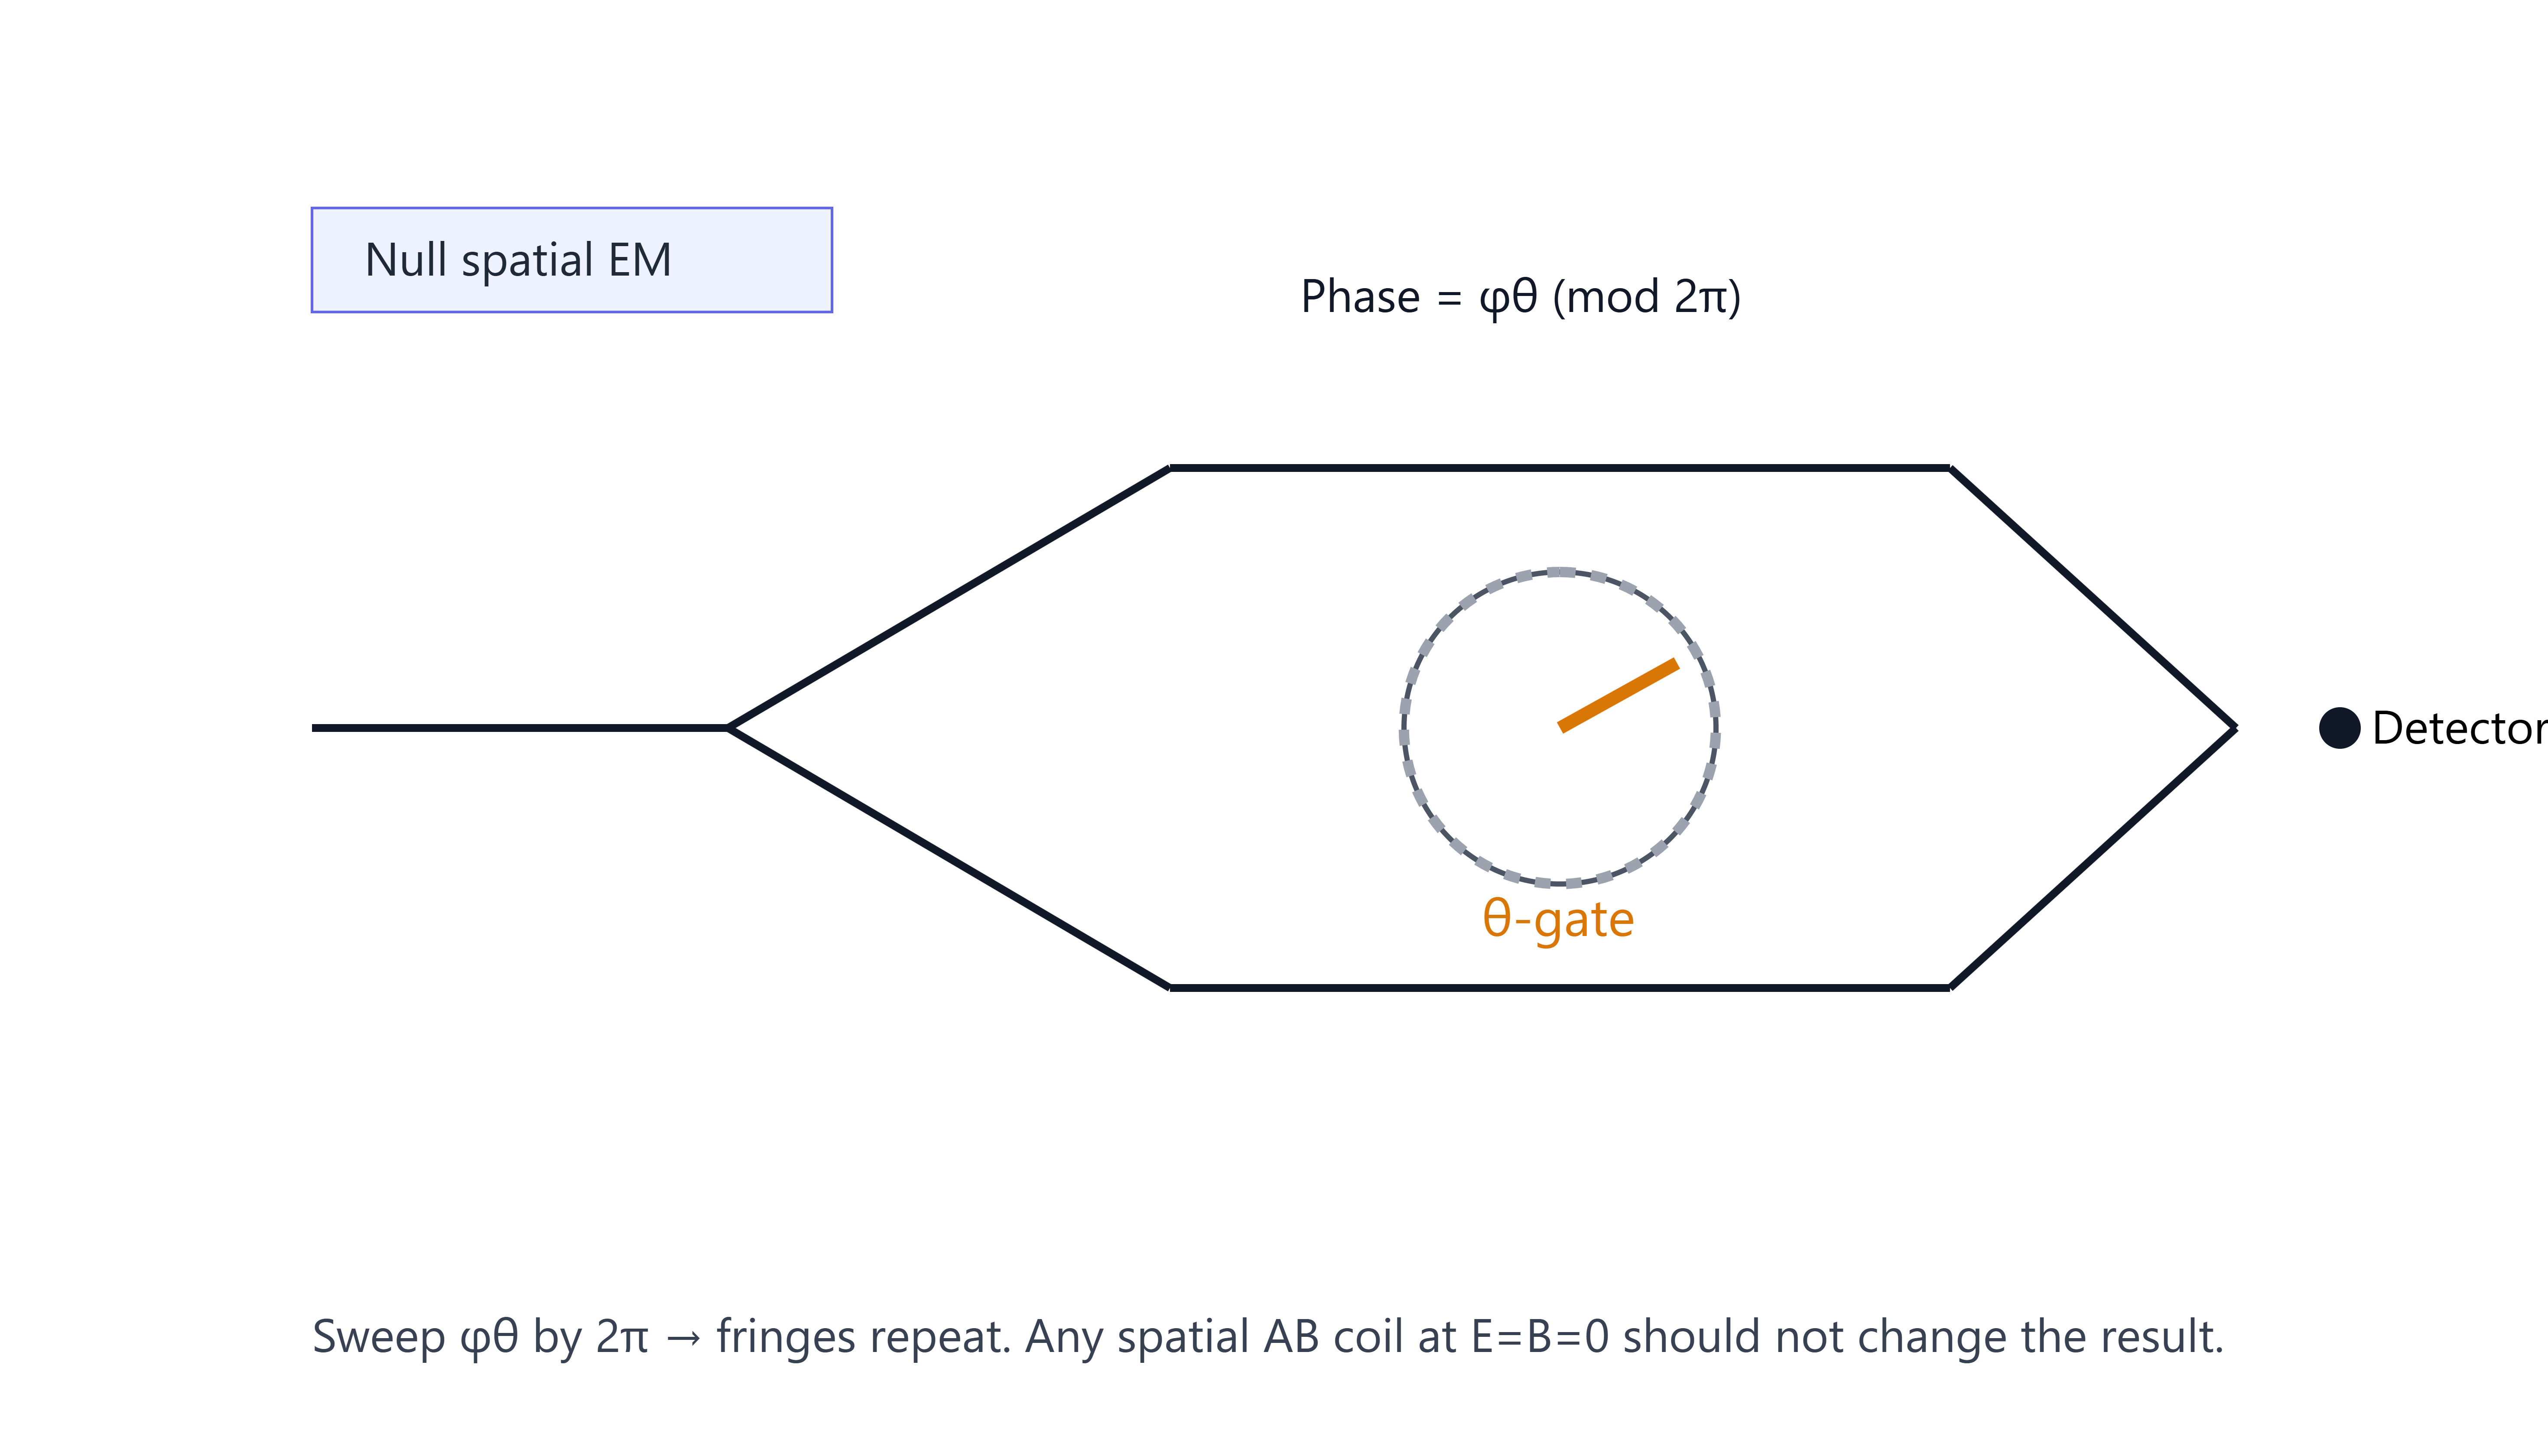
\includegraphics[width=\linewidth]{UG_S3_theta_AB.png}
  \caption{$\theta$--AB interferometer at null spatial EM. The $\theta$-gate dials $\phi_\theta$; fringes are strictly $2\pi$-periodic.}
  \label{fig:theta-ab-cartoon}
\end{figure}

\begin{figure}[htbp]
  \centering
  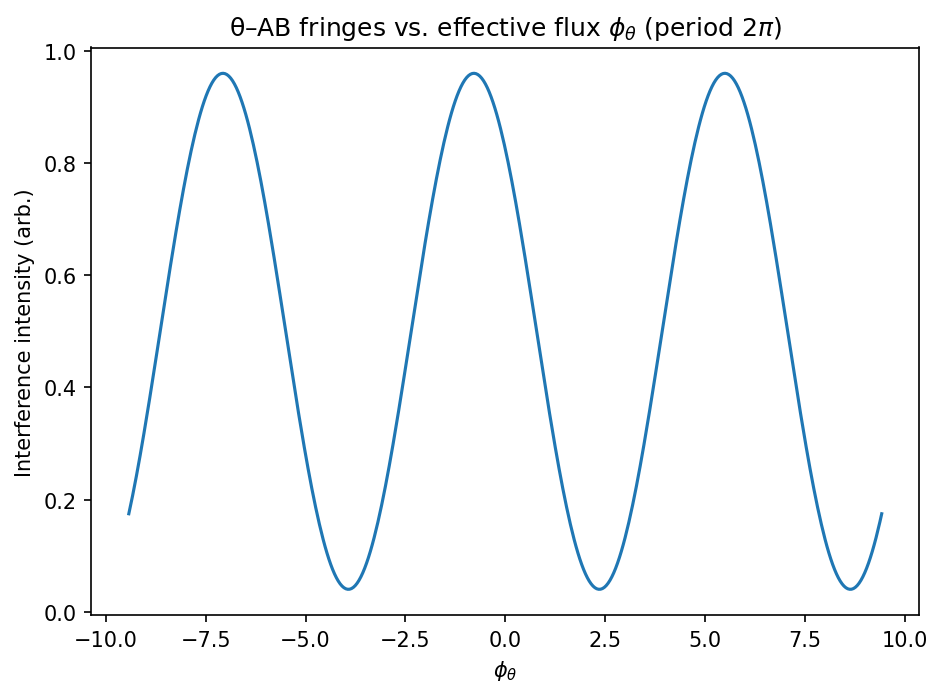
\includegraphics[width=0.7\linewidth]{exp1_fringe_vs_phi.png}
  \caption{Fringe vs. $\phi_\theta$ (simulation).}
  \label{fig:theta-ab-fringe}
\end{figure}

\csvnote{../paper/data/exp1_theta_ab_fringe.csv}

\subsection{Cross-Hall drift from mixed curvature}\label{sec:cross-hall}
With $\bm E=\bm B=0$, $m\ddot X_i = q_\theta\,G_{i\theta}\,\dot\theta$ ($G_{i\theta}=\partial_iA_\theta-\partial_\theta A_i$). For a uniform gate of duration $T$ and nearly constant $\dot\theta$,
\begin{equation}
 \Delta X_i \simeq \alpha\,\frac{q_\theta}{m}\,(\partial_iA_\theta)\,\frac{T^2}{2}\,\dot\theta,\qquad \alpha\lesssim 1.
\end{equation}

\begin{idea}
A hidden current can push a boat sideways. Likewise a gradient $\partial_y A_\theta$ plus a time window with $\dot\theta\neq 0$ nudges the packet: $\Delta y\propto(\partial_y A_\theta)\,\dot\theta\,T^2$. Flip either sign and the drift reverses; turn either off and it vanishes.
\end{idea}

\begin{figure}[htbp]
  \centering
  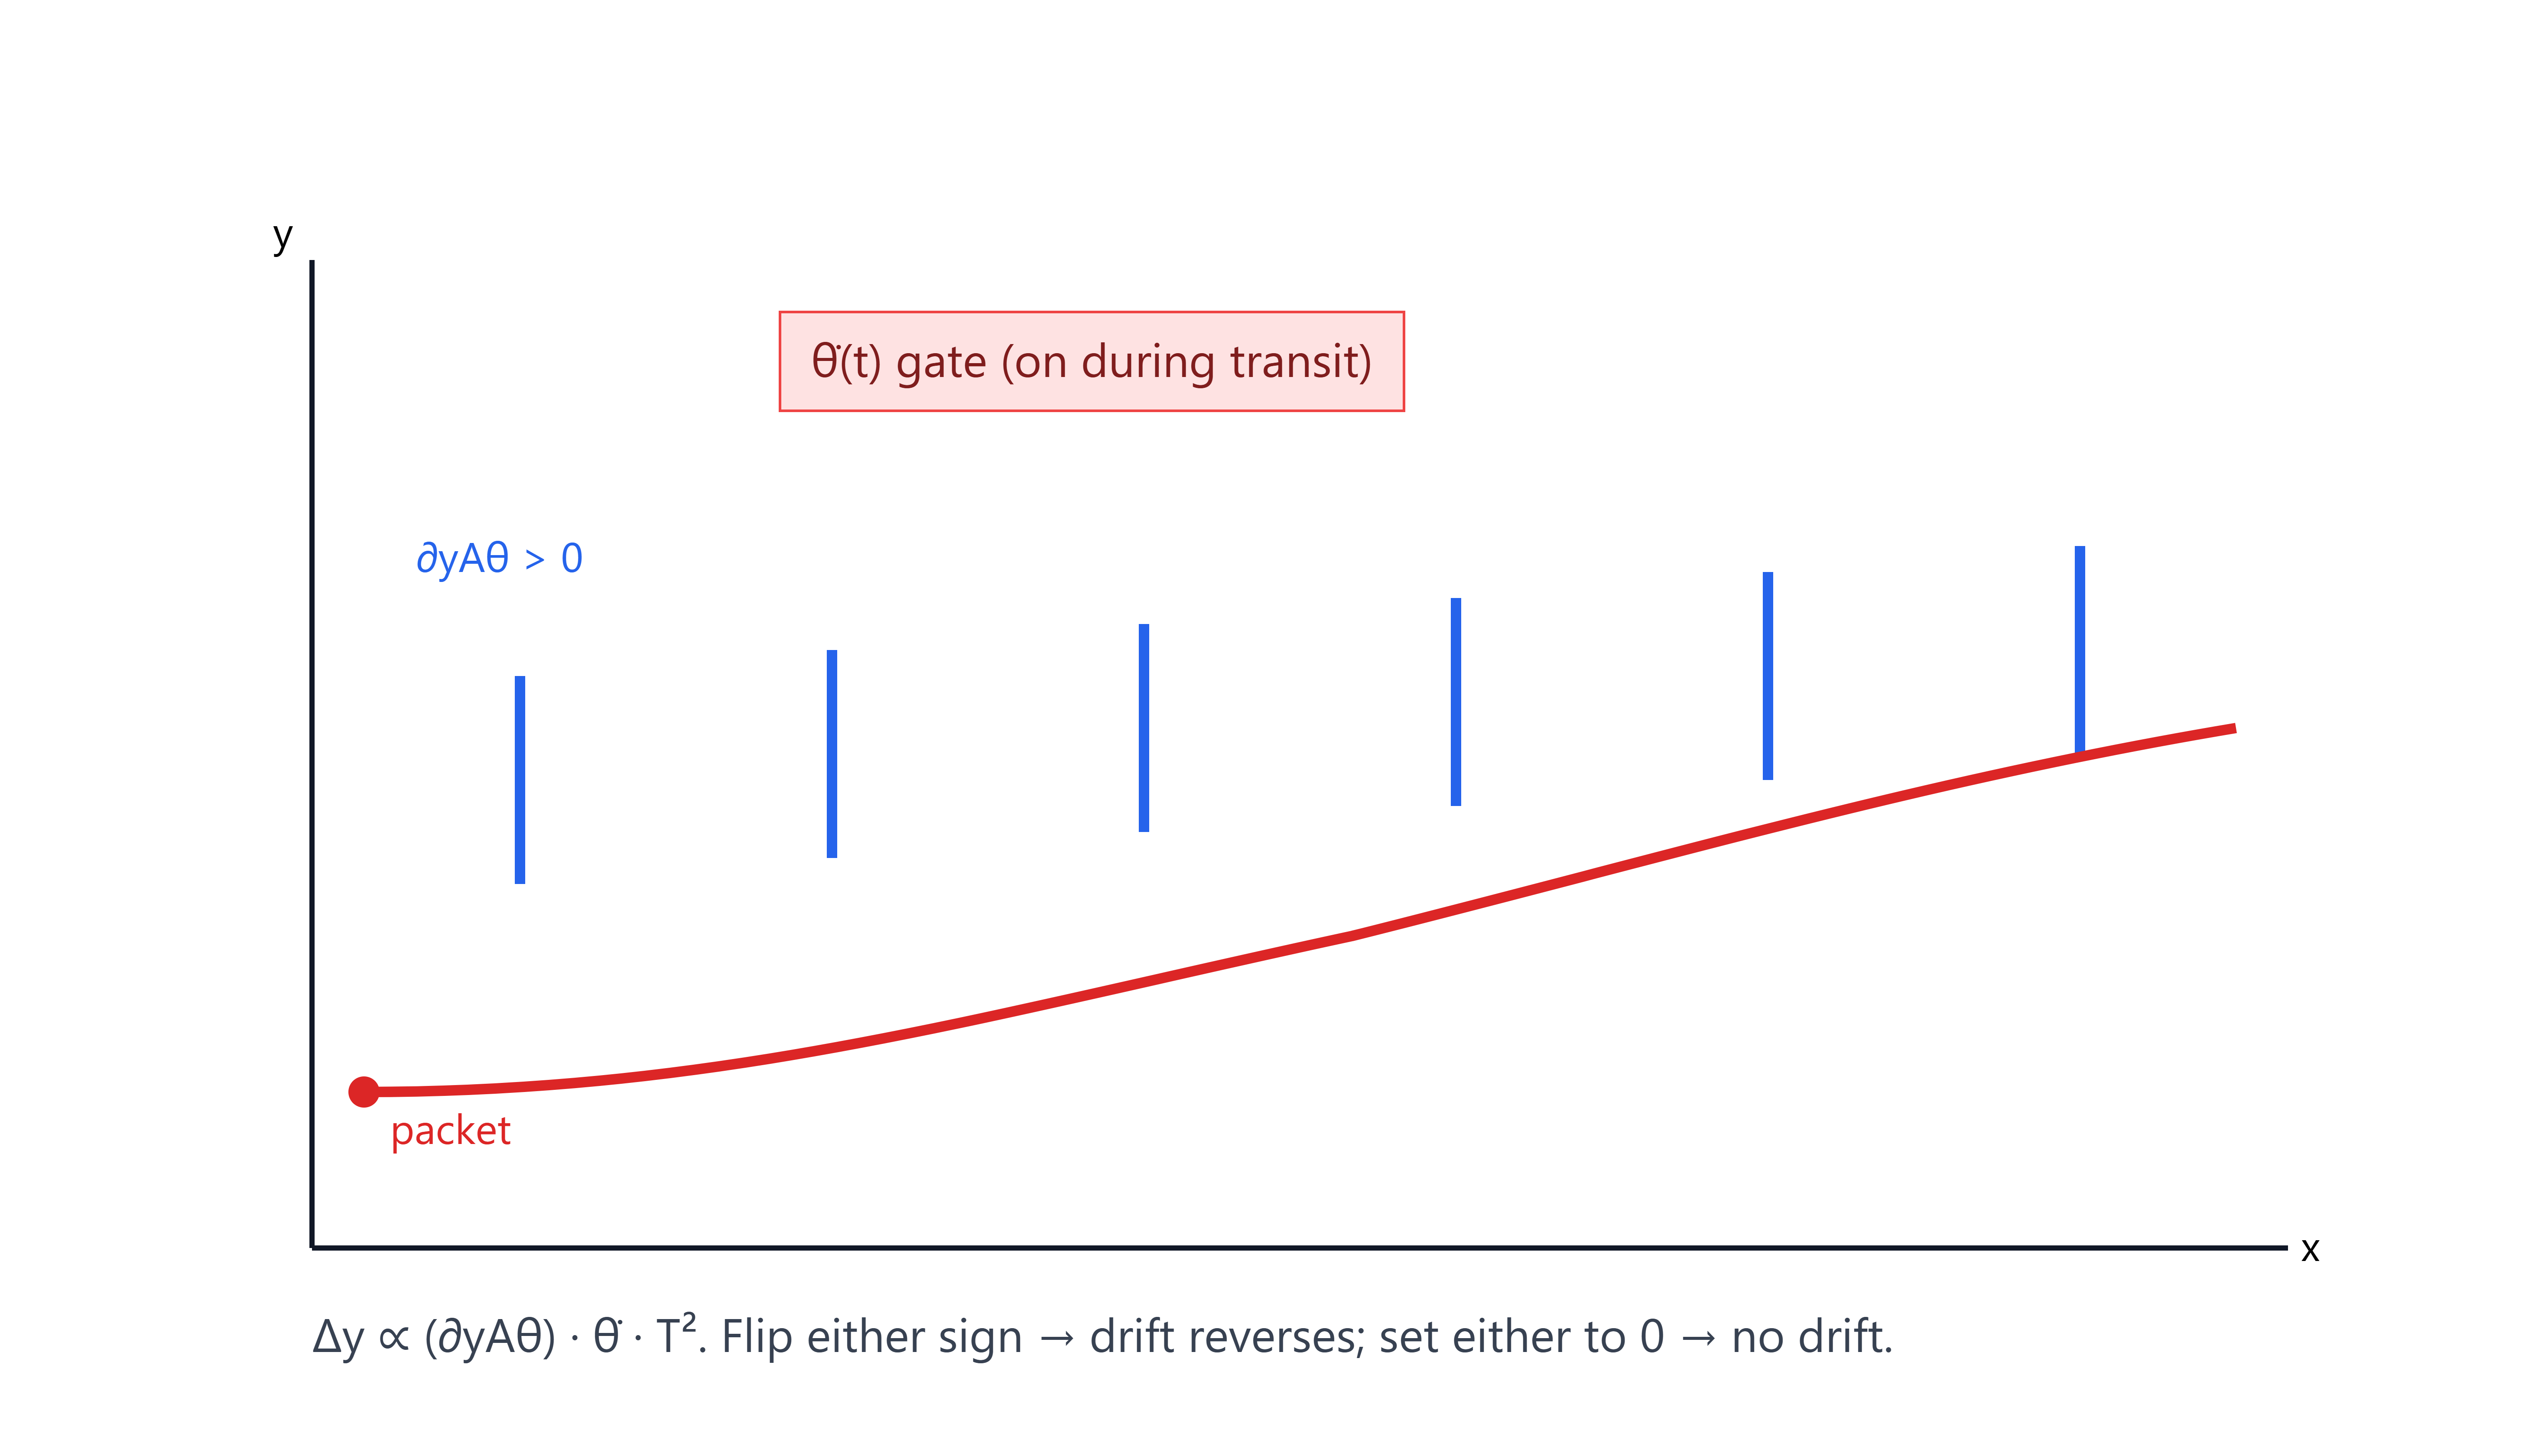
\includegraphics[width=\linewidth]{UG_S3_cross_hall.png}
  \caption{Cross\textendash Hall drift intuition: blue arrows for $\partial_yA_\theta$, red packet deflection.}
  \label{fig:cross-hall-cartoon2}
\end{figure}

\begin{figure}[htbp]
  \centering
  \begin{subfigure}[b]{0.48\linewidth}
    \centering
    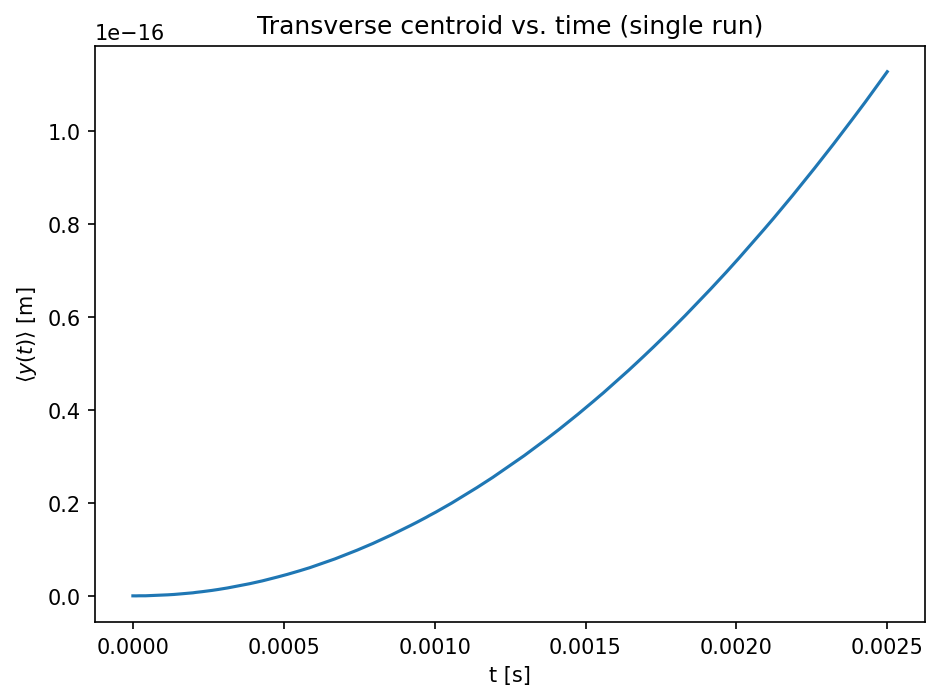
\includegraphics[width=\linewidth]{exp2_y_traj.png}
    \caption{Centroid trajectory $\langle y(t)\rangle$}
    \label{fig:cross-hall-traj}
  \end{subfigure}\hfill
  \begin{subfigure}[b]{0.48\linewidth}
    \centering
    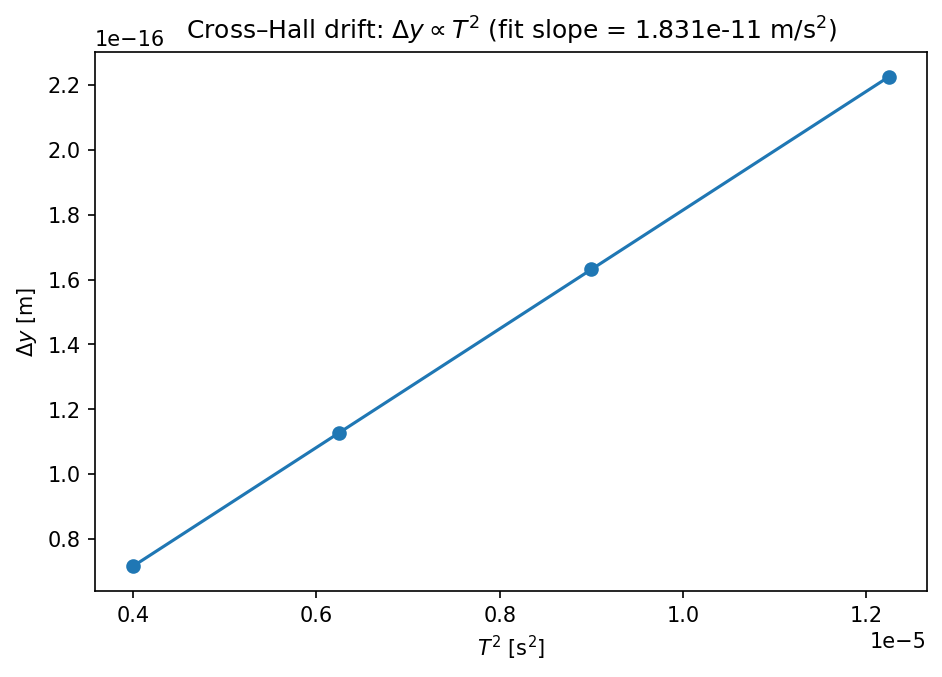
\includegraphics[width=\linewidth]{exp2_dy_vs_T2.png}
    \caption{$\Delta y$ vs $T^2$ scaling}
    \label{fig:cross-hall-scaling}
  \end{subfigure}
  \caption{Cross\textendash Hall drift: simulation traces and $T^2$ scaling.}
  \label{fig:cross-hall}
\end{figure}

\csvnote{../paper/data/exp2_drift_T2.csv}

\subsection{Sidebands from the rotor Hamiltonian}\label{sec:sidebands}
Separating variables $\Psi=\sum_{\ell}\psi_\ell(X)e^{i\ell\theta}$ yields rotor levels $E_\ell=\frac{\hbar^2}{2I}(\ell-\phi_\theta/2\pi)^2$ and nearest-neighbor spacing $\Delta E\approx\hbar^2/(2I)$.

\begin{figure}[htbp]
  \centering
  \begin{subfigure}[b]{0.48\linewidth}
    \centering
  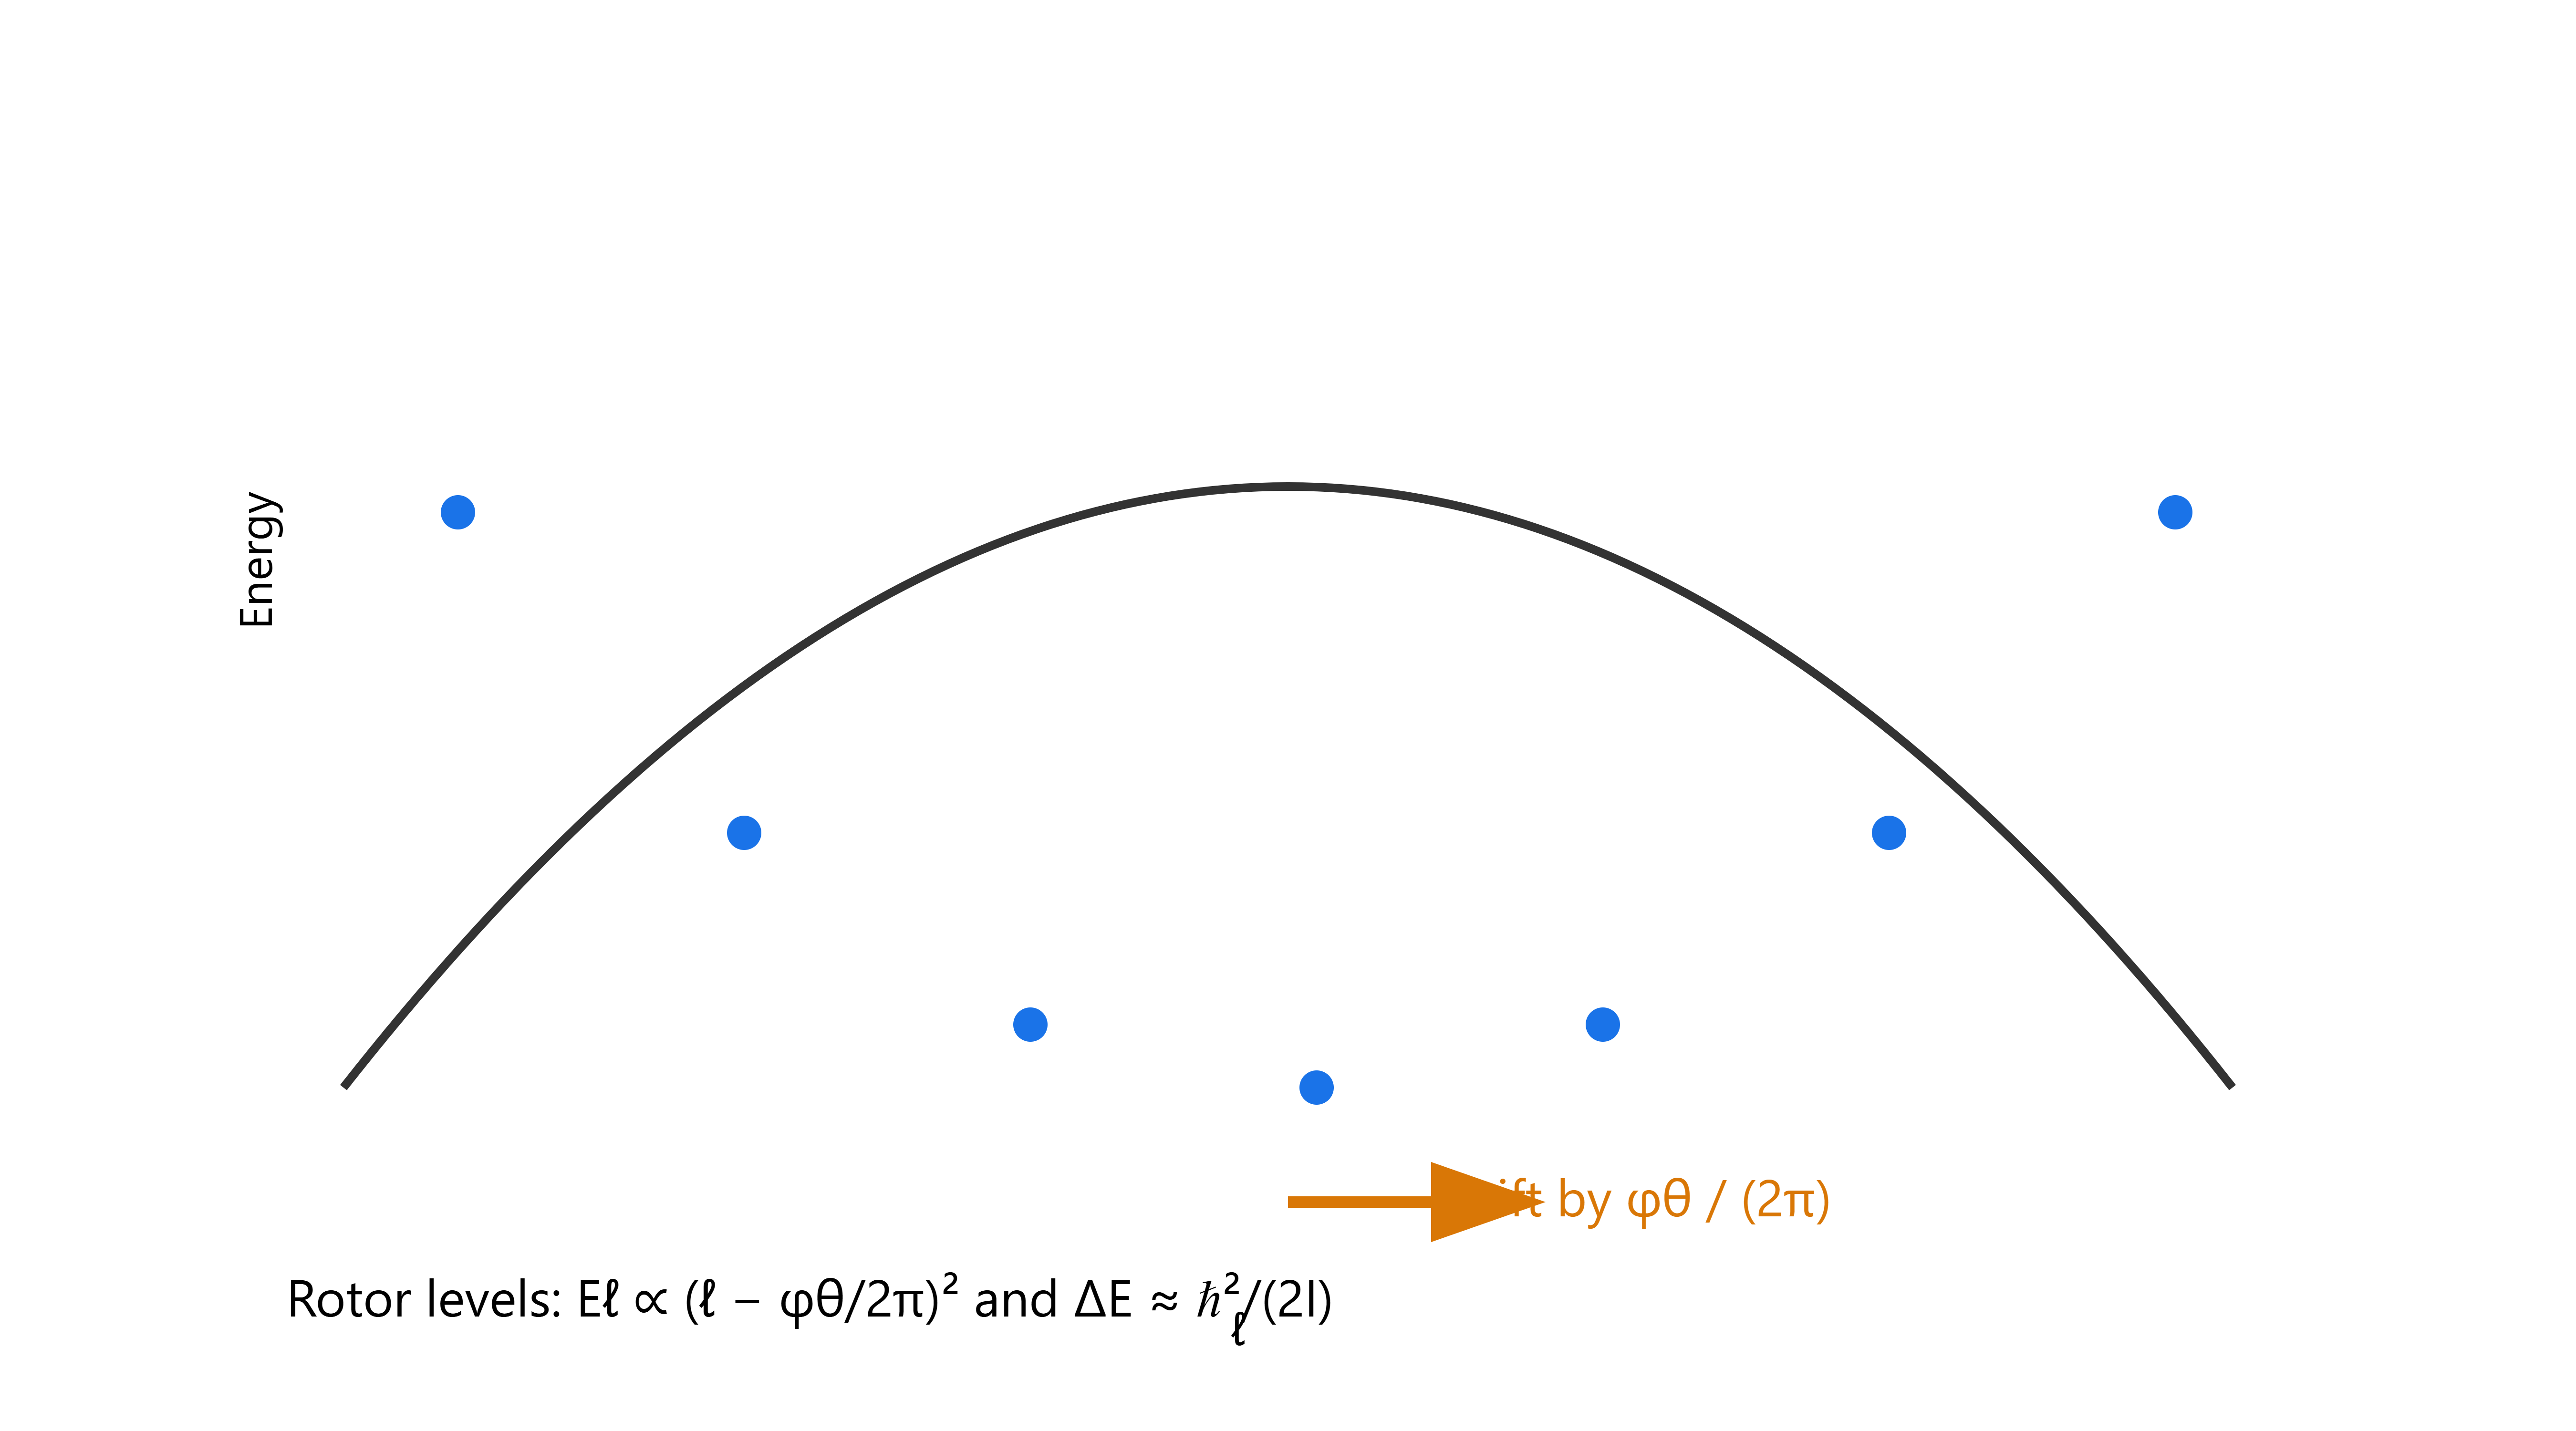
\includegraphics[width=\linewidth]{S3_rotor_levels_cartoon.png}
    \caption{Rotor levels (cartoon)}
    \label{fig:rotor-cartoon}
  \end{subfigure}\hfill
  \begin{subfigure}[b]{0.48\linewidth}
    \centering
    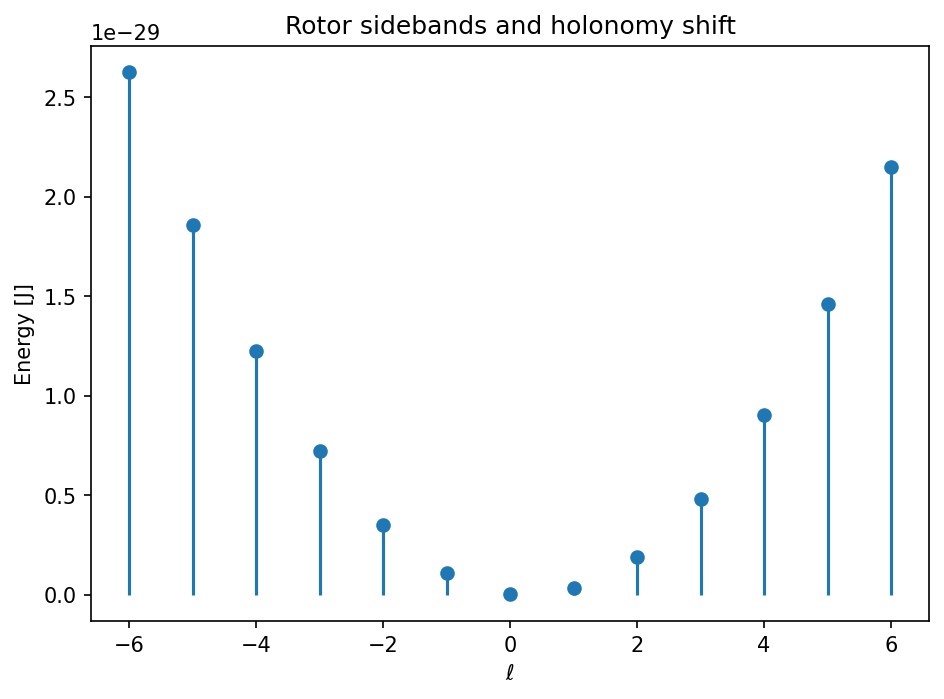
\includegraphics[width=\linewidth]{exp3_rotor_levels.png}
    \caption{Rotor levels (simulation)}
    \label{fig:rotor-sim}
  \end{subfigure}
  \begin{subfigure}[b]{0.48\linewidth}
    \centering
  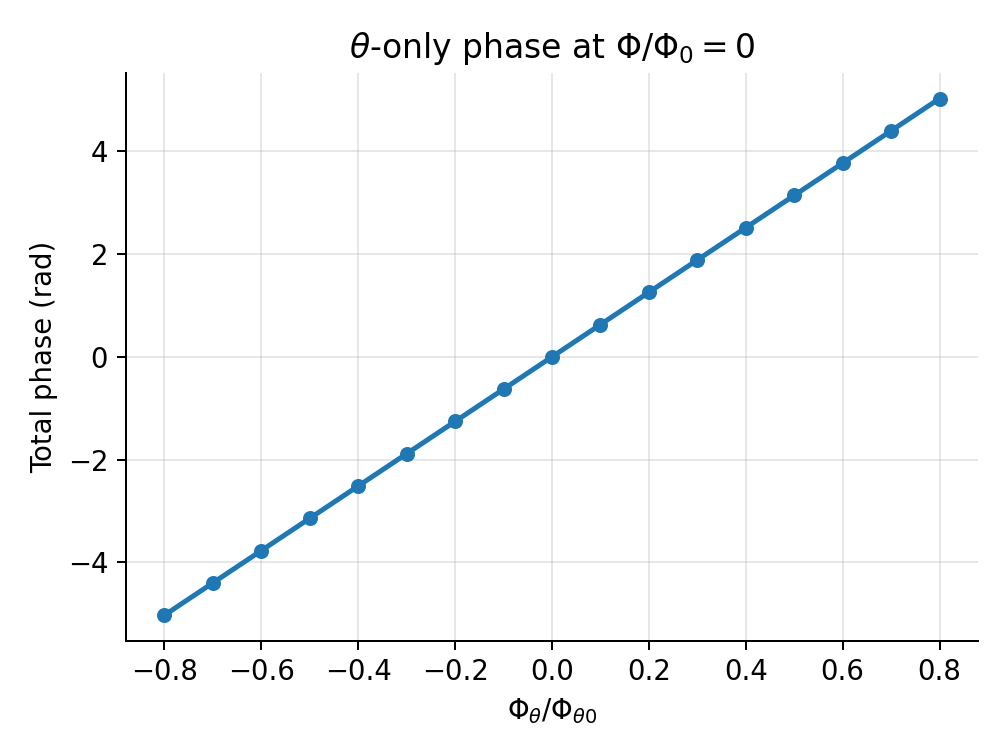
\includegraphics[width=\linewidth]{theta_only.png}
    \caption{$\theta$-only baseline}
    \label{fig:theta-only}
  \end{subfigure}
  \caption{Rotor sidebands and $\theta$-only baseline.}
  \label{fig:rotor}
\end{figure}

\csvnote{../paper/data/exp3_rotor_levels.csv}

\subsection{Order-of-magnitude anchors for \texorpdfstring{$I$}{I}}\label{sec:iom}
$\Delta E=h\,\Delta f$, $\ I\approx \hbar^2/(2\,\Delta E)$. Example: $\Delta f=\SI{1}{Hz}\Rightarrow I\approx 8.4\times 10^{-36}\,\mathrm{J\,s^2}$.

\subsection{Falsification protocol}\label{sec:falsification}
Vary spatial flux at fixed $\phi_\theta$; enforce $2\pi$ periodicity in $\phi_\theta$; use closed $\theta$-loop controls and arm swaps.

\subsection{Consistency checks \& limits (QM/NR)}\label{sec:lab-consistency}
Fiber-off ($I\to\infty$, $q_\theta\to 0$), pure $\theta$ sector ($q_X\to 0$), large-gauge periodicity in $\oint A_\theta d\theta$.

\subsection{Methods: \texorpdfstring{$\theta$}{theta}--Aharonov--Bohm interferometer}\label{sec:methods-theta-ab}
Program a $\theta(t)$ modulation that advances by $2\pi N_\theta$ during the arm transit; if $A_\theta$ is approximately constant along the path in $\theta$, then $\Delta\phi_\theta \approx (q_\theta/\hbar) A_\theta (2\pi N_\theta)$.

\begin{figure}[htbp]
  \centering
  \begin{subfigure}[b]{0.48\linewidth}
    \centering
  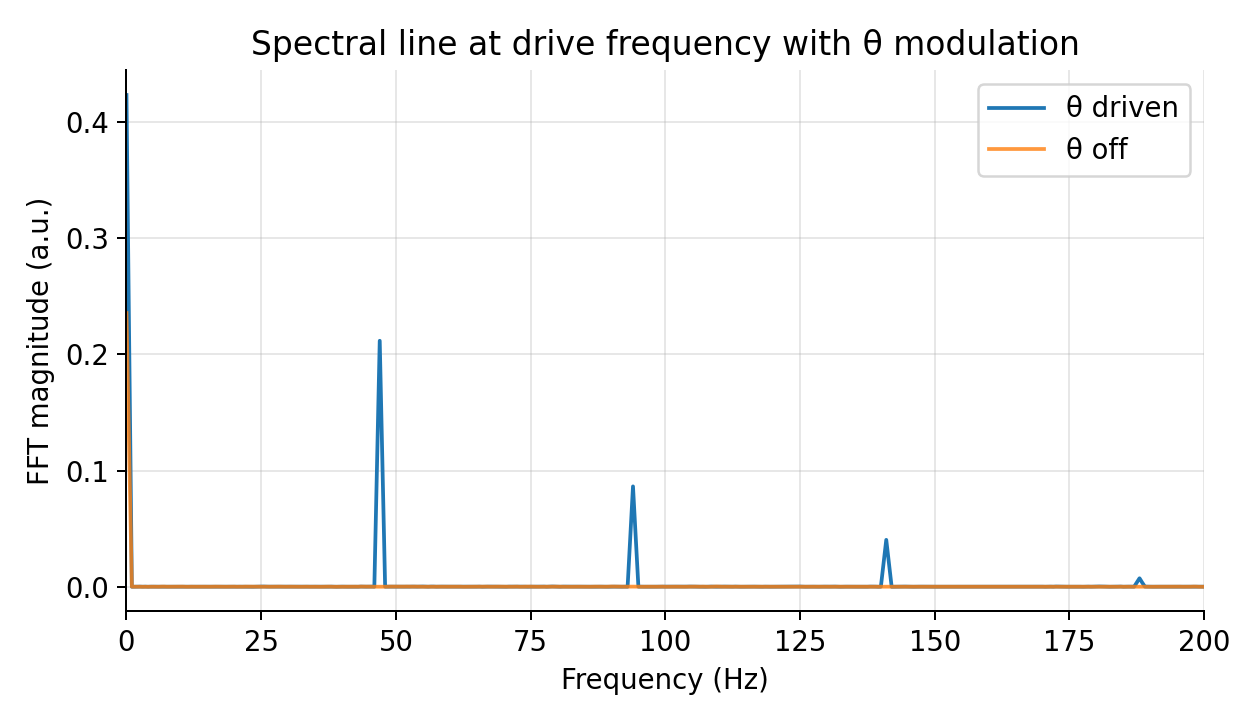
\includegraphics[width=\linewidth]{fft_theta_drive.png}
    \caption{FFT of a sample $\theta$ drive}
    \label{fig:fft-theta}
  \end{subfigure}\hfill
  \begin{subfigure}[b]{0.48\linewidth}
    \centering
  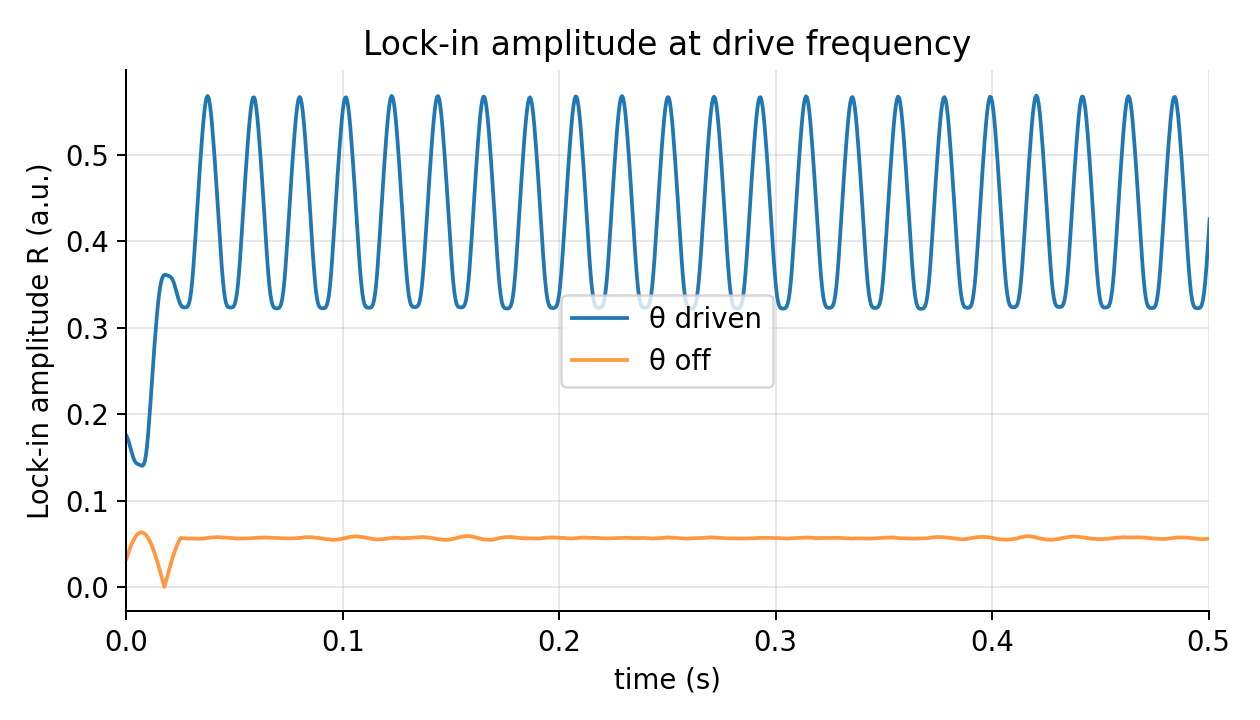
\includegraphics[width=\linewidth]{lockin_theta_drive.png}
    \caption{Lock-in demodulation concept}
    \label{fig:lockin-theta}
  \end{subfigure}
  \caption{Method visuals for $\theta$--AB interferometry.}
  \label{fig:methods}
\end{figure}

\subsection{Mesoscopic Transport: AB Rings with a \texorpdfstring{$\theta$}{theta}-Flux Offset}\label{sec:mesoscopic}
$G(\Phi,\Phi_\theta)\propto \cos[2\pi(\Phi/\Phi_0+\Phi_\theta/\Phi_{\theta,0})]$, $\Phi_{\theta,0}=2\pi\hbar/q_\theta$.

\subsection{Singularity seam: where classical GR fails and QM fixes}\label{sec:singularity-seam}
Classical FRW: stiff $a^{-6}$ alone doesn’t bounce; adding curvature ($-k/a^2$ with $k>0$) creates a turning point. Wheeler--DeWitt adds a repulsive $+C/a^2$ barrier that blocks $a\to 0$.
